\section{Device Discovery}
\subsection{Purpose}
In order for proposed system to have an efficient filtering function. First,
it must be able to percieve how many devices are operating, what is their IP address and MAC address.
This data are crucial, it serves as a profile of what should the system pay attention to.  

\subsection{Method}
We have tested our host detection algorithm constructed with three approaches: Detecting hosts by ARP request, by ARP reply and by gratuitous ARP.
\begin{itemize}
    \item \textbf{ARP request} is Arp packet with opcode equal to 1 and Target MAC address equal to “00:00:00:00:00:00”. We considered Sender of this packet to be host in LAN and added tuple of its MAC address (SHA) and IP address (SPA) to host list.
    \item \textbf{ARP reply} is Arp packet with opcode equal to 2. We added both Target and Sender of this packet to host list. 
    \item \textbf{Gratuitous ARP} is Arp packet which has is sender IP address equal to target IP address, its opcode equal to 1, and has target MAC address equal to “00:00:00:00:00:00”. We added Sender of this packet it to host list.  
\end{itemize}

All three approaches had been tested using both pattern A and B packet data. 

\subsection{Result}
Result of device discovery is shown in figure \ref{fig:s4_device_discovery_result}. From the result we knew that Gratuitous ARP approach performed poorly in most case, detecting no device or unrelated device. While, both ARP Reply approach and ARP request approach were able to detect some hosts.

\begin{figure}[H]
    \centering
    \begin{subfigure}[b]{0.25\textwidth}
        \centering
        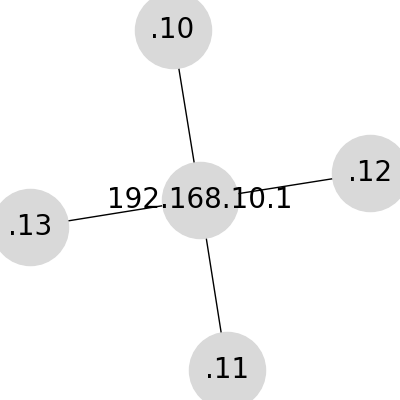
\includegraphics[width=\textwidth]{device_detection/eroom_switch_req}
        \caption{eroom + Pattern A + ARP Request}
        \label{fig:s4_eroom_a_req}
    \end{subfigure}
    \hfill
    \begin{subfigure}[b]{0.25\textwidth}
        \centering
        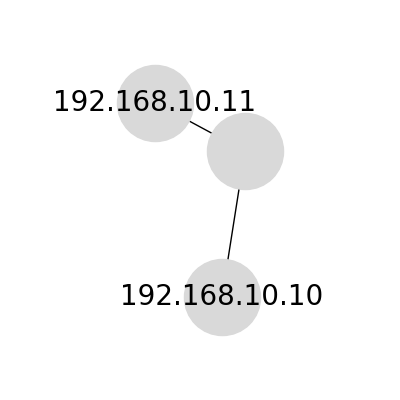
\includegraphics[width=\textwidth]{device_detection/eroom_switch_rep}
        \caption{eroom + Pattern A + ARP Reply}
        \label{fig:s4_eroom_a_rep}
    \end{subfigure}
    \hfill
    \begin{subfigure}[b]{0.25\textwidth}
        \centering
        
\includegraphics[width=\textwidth]{device_detection/eroom_switch_gra}
        \caption{eroom + Pattern A + Gratuitous ARP}
        \label{fig:s4_errom_a_gra}
    \end{subfigure}
    \newline 
    \begin{subfigure}[b]{0.25\textwidth}
        \centering
        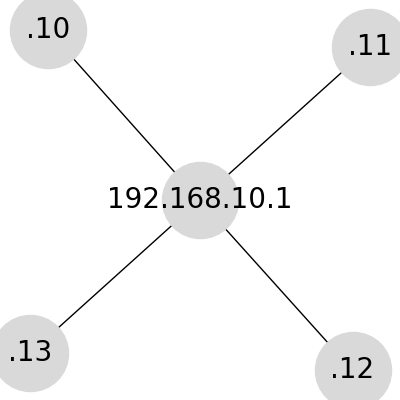
\includegraphics[width=\textwidth]{device_detection/eroom_arp_req}
        \caption{eroom + Pattern B + ARP Request}
        \label{fig:s4_10f_b_req}
    \end{subfigure}
    \hfill
    \begin{subfigure}[b]{0.25\textwidth}
        \centering
        
\includegraphics[width=\textwidth]{device_detection/eroom_arp_rep}
        \caption{eroom + Pattern B + ARP Reply}
        \label{fig:s4_eroom_b_rep}
    \end{subfigure}
    \hfill
    \begin{subfigure}[b]{0.25\textwidth}
        \centering
        
\includegraphics[width=\textwidth]{device_detection/eroom_arp_gra}
        \caption{eroom + Pattern B + Gratuitous ARP}
        \label{fig:s4_eroom_b_gra}
    \end{subfigure}

    \caption{The result of device discovery}
    \label{fig:s4_device_discovery_result}
\end{figure}

\subsection{Discussion}
From the result, we found that the best approach to find devices in the system is to analyze ARP Request packet. 
The reason ARP reply didn’t perform as well as the Request pattern is because air conditioners were connected to the router wirelessly,
 therefore we couldn’t collect it ARP reply packet directly. We believe that if all devices were connected to the switch through ethernet cable. The ARP reply approach should perform as well as the ARP request pattern.  
 
ARP reply might seem like a not efficient method, considering that our bridge PC needs to have network interface at least equal to the number of devices plus the switch. However, if the system was implemented with SDN-switch (Software Defined Network switch), we can easily sniff through all packet. We can set a rule in SDN-controller plane to copy all ARP reply packet in network plane.